\documentclass[20pt,a4paper]{article}
\usepackage{fullpage}
\usepackage{amsmath}
\usepackage{amssymb}
\usepackage[usenames]{color}
\usepackage{graphicx}
\usepackage{amsmath}
\usepackage{array}
\usepackage{hyperref}
\usepackage[noadjust]{cite}
%\usepackage{program}
\usepackage{caption}
\usepackage{subcaption}
\usepackage{subfloat}
\usepackage{framed}
\usepackage{color}
%\usepackage{CJKutf8}
\usepackage{geometry}
\usepackage[BoldFont,SlantFont,CJKchecksingle]{xeCJK}%---------------------------使用xeCJK宏包
\leftmargin=0.25in
\oddsidemargin=0.15in
\textwidth=6.0in
\topmargin=-0.8in
\textheight=19in

\raggedright
\pagenumbering{arabic}
\geometry{top=0.5cm}
\geometry{bottom=0.5cm}

\def\bull{\vrule height 0.8ex width .7ex depth -.1ex }
% DEFINITIONS FOR RESUME

\newenvironment{changemargin}[2]{%
  \begin{list}{}{%
    \setlength{\topsep}{0pt}%
    \setlength{\leftmargin}{#1}%
    \setlength{\rightmargin}{#2}%
    \setlength{\listparindent}{\parindent}%
    \setlength{\itemindent}{\parindent}%
    \setlength{\parsep}{\parskip}%
  }%
  \item[]}{\end{list}
}

\newcommand{\lineover}{
	\begin{changemargin}{-0.05in}{-0.05in}
		\vspace*{-8pt}
		\hrulefill \\
		\vspace*{-2pt}
	\end{changemargin}
}

\newcommand{\header}[1]{
	\begin{changemargin}{-0.5in}{-0.5in}
		\scshape{#1}\\
  	\lineover
	\end{changemargin}
}

\newcommand{\contact}[4]{
	\begin{changemargin}{-0.5in}{-0.5in}
		\begin{center}
			{\large \scshape {#1}}\\ %\smallskip
			{#2}\\ %\smallskip
			{#3}\\ %\smallskip
			{#4}%\smallskip
		\end{center}
	\end{changemargin}
}
%\newcommand{\lineunder}{\vspace*{-8pt} \\ \hspace*{-18pt} \hrulefill \\}
%\newcommand{\contact}[3]{
%\vspace*{-8pt}
%\begin{center}
%{\LARGE \scshape {#1}}\\
%#2 \lineover
%#3
%\end{center}
%\vspace*{-8pt}
%}


\newenvironment{body} {
	\vspace*{-16pt}
	\begin{changemargin}{-0.25in}{-0.5in}
  }	
	{\end{changemargin}
}	

\newcommand{\school}[4]{
	\textbf{#1} \hfill \emph{#2\\}
	#3\\
	#4\\
}
\newcommand*{\linkedin}[1]{\def\@linkedin{#1}}
% END RESUME DEFINITIONS

\begin{document}

%\begin{CJK}{UTF8}{gbsn}
%%%%%%%%%%%%%%%%%%%%%%%%%%%%%%%%%%%%%%%%%%%%%%%%%%%%%%%%%%%%%%%%%%%%%%%%%%%%%%%%
% Name
%\contact{张猛}{Email:zhangmeng0778@gmail.com}{Tel:14714307955}
\begin{figure}[t]
	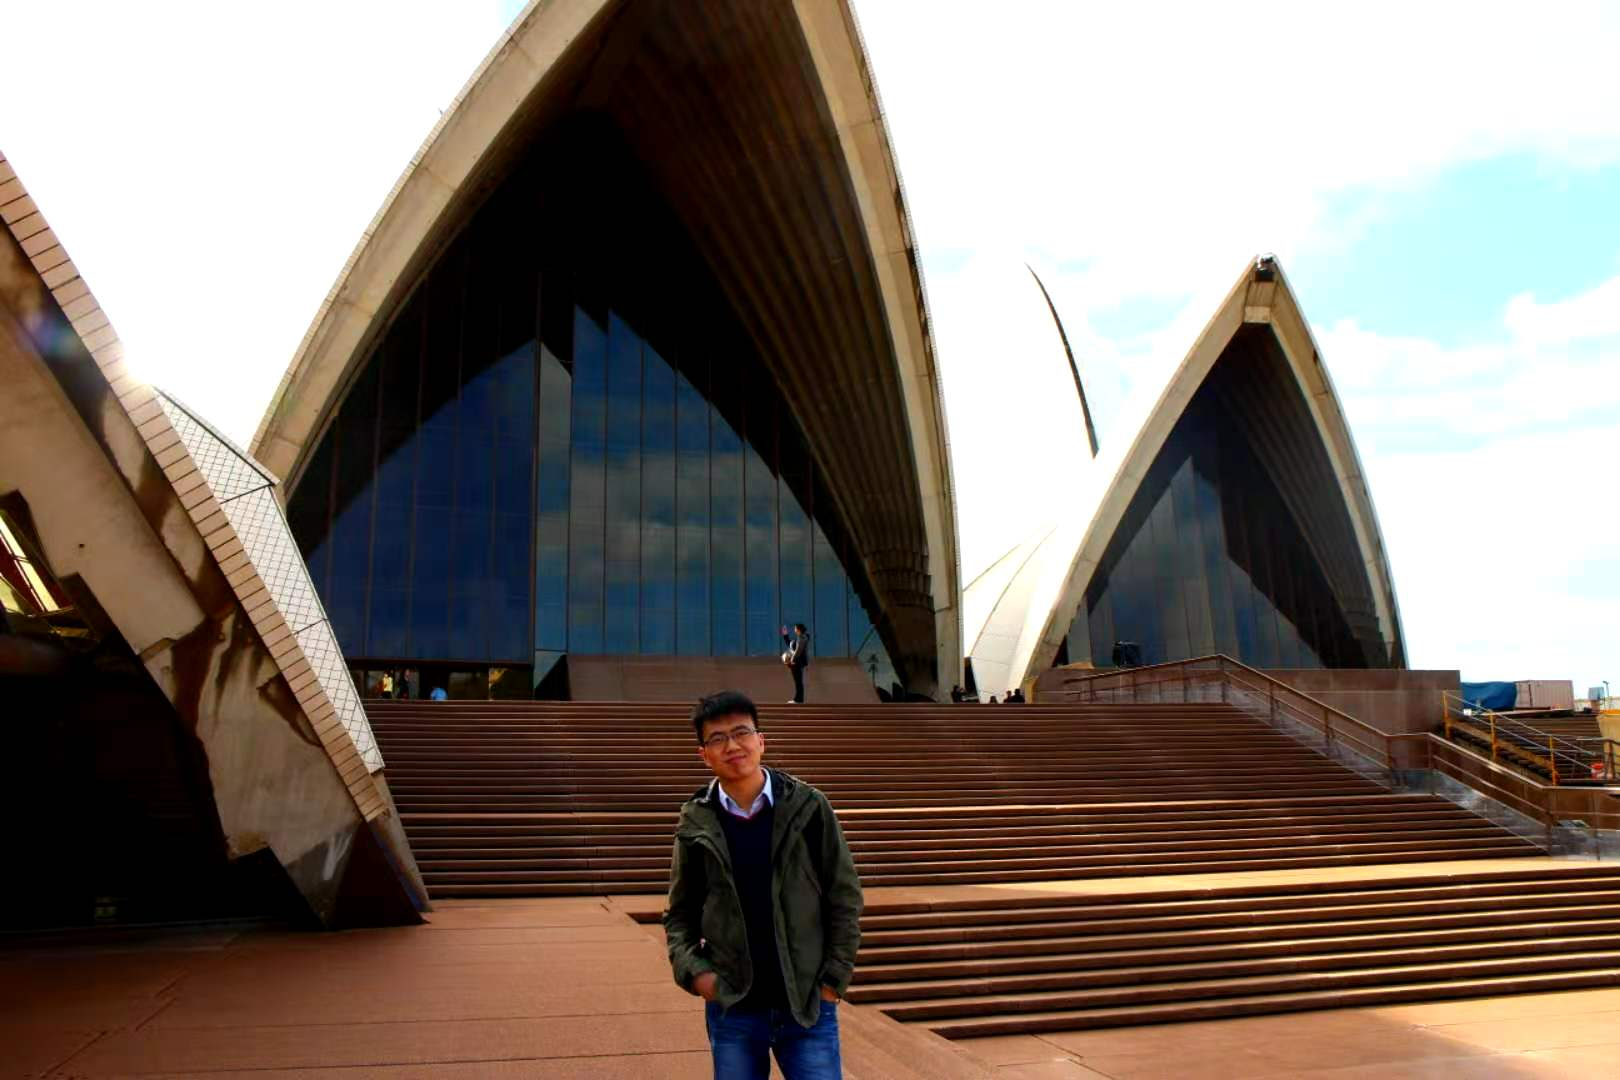
\includegraphics[scale=0.2]{./cover.jpeg}
\end{figure}
\begin{minipage}[t]{0.5\textwidth}
\textbf{张猛} \\
\hfill 专业领域: 推荐、广告、机器学习\\
\end{minipage}
%
\begin{minipage}[t]{0.48\textwidth}
\textsc{Email:} zhangmeng0778@qq.com \\
\end{minipage}

\header{关于自己}
\begin{body}
	\vspace{14pt}
	百度, 北京\\
	\begin{itemize}
		\item \textbf{推荐广告}  \hfill \emph{} \\
	\end{itemize}
	硕士, 香港中文大学, 香港\\
	\begin{itemize}    
    		\item 计算机科学工程系 \hfill \emph{} \\
	\end{itemize}
	本科, 厦门大学, 福建\\
	\begin{itemize}
		\item 计算机科学与技术系  \hfill \emph{} \\
	\end{itemize}
\end{body}

\header{介绍}
\begin{body}
	\vspace{14pt}
	人生目标是做一番事业, 驾长车,踏破贺兰山缺\\
	喜欢的哲学: 辩证唯物主义、庄子哲学\\
	兴趣爱好: 读书、写作、engineering、商业、科技
\end{body}

\header{工程师的技能栈}
\begin{body}
	\vspace{14pt}
	技术方向: 推荐系统、排序模型、机制 \\
	编程语言:{} python, pandas, shell, C++, C \\
	模型框架:{} Paddle、Tensorflow\\
\end{body}

\header{做过的一些事}
\begin{body}
	\vspace{14pt}
	在百度为其实现了商业广告由传统点击模式向转化模式的转变, 做成了几项大幅提升广告营收的技术创新 \\
	提升百度地图完成实时公交产品的市场覆盖, 实现了少有的LBS大数据挖掘的产品化\\
\end{body}

\header{可公开的写作}
\begin{body}
	\vspace{14pt}
	人生思考: \url{https://sheldonzhang.github.io/thinking} \\
	日常技术笔记: \url{https://sheldonzhang.github.io/tech} \\
	日记: 进步来源于实践,更来源于日常的思考和反省。自己每天都坚持日记,由于涉及到具体的人和事,所以就不公开了。
\end{body}


\header{过去些许的奖励}
\begin{body}
	\vspace{14pt}
	百度: 百度最高奖还有其它十几项奖 \hfill{} \emph{}\\
    硕士: 全额奖学金(HK postgraduate studentship) \hfill{} \emph{} \\
    本科: ACM亚洲区域赛银奖、Scilab一等奖还有其它十几项奖 \hfill{} \emph{}\\
\end{body}

\header{联系我}
\begin{body}
	\vspace{14pt}
	欢迎同行、同道的朋友们联系我,聊技术聊人生聊合作\\
	\begin{figure}[h]
		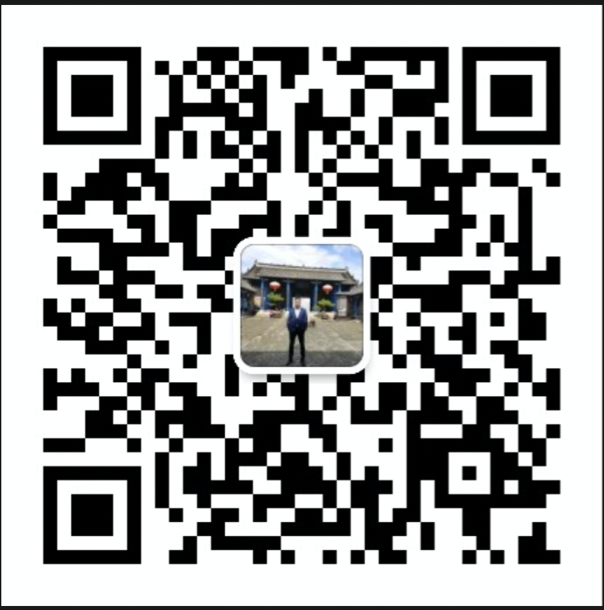
\includegraphics[scale=0.2]{./weixin_qcode.png}
	\end{figure}
\end{body}

%%%%%%%%%%%%%%%%%%%%%%%%%%%%%%%%%%%%%%%%%%%%%%%%%%%%%%%%%%%%%%%%%%%%%%%%%%%%%%%%
% Awards and Honors


\end{document} 
